\section{Mengenlehre}
\subsection*{Teilmenge und Obermenge}
Eine Menge $B$ heißt Teilmenge einer Menge $A$ genau dann,
wenn jedes Element von $B$ auch ein Element von $A$ ist ($B\subseteq A\Leftrightarrow\forall x:x\in B\Rightarrow x\in A$).
$A$ heißt dann Obermenge von $B$. Eine Menge $B$ heißt echte Teilmenge von $A$ ($B\subset A$), falls gilt $B\subseteq A\wedge B\neq A$
\subsection*{Grundlegende Mengenoperationen}
Seien $M, N$ Mengen und sei $U$ die Grundmenge.\\
Vereinigungsmenge:\\
$M\cup N:=\{x\mid x\in M\vee x\in N\}$\\
Schnittmenge:\\
$M\cap N:=\{x\mid x\in M\wedge x\in N\}$\\
Differenz:\\
$M\setminus N:=\{x\mid x\in M\wedge x\notin N\}$\\
Disjunkte Menge: $M\cap N=\emptyset$
\subsection*{Potenzmenge}
Sei $M$ eine Menge. Die Menge aller Teilmengen von $M$ heißt Potenzmenge von $M$ und
wird $\mathcal{P}(M)$ notiert: $\mathcal{P}(M):=\{X\mid X\subseteq M\}$\\
\emph{Beispiel:}\\
$\mathcal{P}(\{a,b\})=\{\emptyset,\{a\},\{b\},\{a,b\}\}$\\
$\mathcal{P}(\emptyset)=\{\emptyset\}$\\
$\mathcal{P}(\{\emptyset\})=\{\emptyset,\{\emptyset\}\}$\\
$\mathcal{P}(\mathcal{P}(\mathcal{P}(\emptyset)))=\{\emptyset,\{\emptyset\},\{\{\emptyset\}\},\{\emptyset,\{\emptyset\}\}\}$
\subsection*{Hassediagramm}
\begin{wrapfigure}[9]{r}{.46\linewidth}
\vspace{-20pt}
\hspace{-0pt}
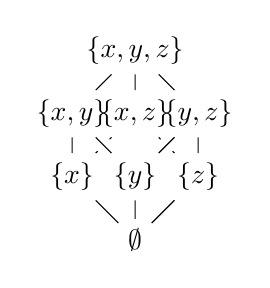
\begin{tikzpicture}[scale=0.4]
  \node (max) at (0,4) {$\{x,y,z\}$};
  \node (a) at (-2,2) {$\{x,y\}$};
  \node (b) at (0,2) {$\{x,z\}$};
  \node (c) at (2,2) {$\{y,z\}$};
  \node (d) at (-2,0) {$\{x\}$};
  \node (e) at (0,0) {$\{y\}$};
  \node (f) at (2,0) {$\{z\}$};
  \node (min) at (0,-2) {$\emptyset$};
  \draw (min) -- (d) -- (a) -- (max) -- (b) -- (f)
  (e) -- (min) -- (f) -- (c) -- (max)
  (d) -- (b);
  \draw[preaction={draw=white, -,line width=6pt}] (a) -- (e) -- (c);
\end{tikzpicture}
\end{wrapfigure}
Man kann die Inklusionsbeziehungen aller Teilmengen in Form eines Hasse-Diagramms veranschaulichen. Das Hasse-Diagramm für $\mathcal{P}(\{x,y,z\})$ lässt sich dann wie folgt darstellen:
\subsection*{Venn-Diagramm}
\begin{tikzpicture}[scale=.45]
    \begin{scope}
        \clip \firstcircle;
        \fill[filled] \secondcircle;
    \end{scope}
    \draw[outline] \firstcircle node {$A$};
    \draw[outline] \secondcircle node {$B$};
    \node[anchor=south] at (current bounding box.north) {$A \cap B$};
\end{tikzpicture}
%Set A or B but not (A and B) also known a A xor B
\begin{tikzpicture}[scale=.45]
\hspace{-.5cm}
    \draw[filled, even odd rule] \firstcircle node {$A$}
                                 \secondcircle node{$B$};
    \node[anchor=south] at (current bounding box.north) {$\overline{A \cap B}$};
\end{tikzpicture}
% Set A or B
\begin{tikzpicture}[scale=.45]
    \draw[filled] \firstcircle node {$A$}
                  \secondcircle node {$B$};
    \node[anchor=south] at (current bounding box.north) {$A \cup B$};
\end{tikzpicture}
% Set A but not B
\hspace{.5cm}
\begin{tikzpicture}[scale=.45]
    \begin{scope}
        \clip \firstcircle;
        \draw[filled, even odd rule] \firstcircle node {$A$}
                                     \secondcircle;
    \end{scope}
    \draw[outline] \firstcircle
                   \secondcircle node {$B$};
    \node[anchor=south] at (current bounding box.north) {$A\setminus B$};
\end{tikzpicture}
\subsection*{Operationen auf Mengenfamilien}
Sei $\mathcal{F}=\{\{1,2,3,4\},\{3,4,5,6\}\}$ Mengenfamilie.
Vereinigung aller Mengen aus $\mathcal{F}$:\\
$\bigcup\mathcal{F}=\{1,2,3,4,5,6\}$\\
Durchschnitt aller Mengen aus $\mathcal{F}$:\\
$\bigcap\mathcal{F}=\{3,4\}$
\subsection*{Kartesisches Produkt}
Seien $A,B$ Mengen, dann ist das kartesische Produkt (Kreuzprodukt)
von $A$ und $B$ definiert als: $A\times B:=\{(a,b)\mid a\in A\wedge b\in B\}$. 
$A\times B$ ist die Menge aller geordneten Paare von $A$ und $B$.\\
\emph{Hinweis:}\\
$(a,b)=(c,d)\Leftrightarrow a=c\wedge b=d$\\
$A\times\emptyset=\emptyset\times A=\emptyset$\\
$A\times B\neq B\times A$\\
\emph{Beispiel:}\\
$\{1,2\}\times\{3,4\}=\{(1,3),(1,4),(2,3),(2,4)\}$\\
$\{3,4\}\times\{1,2\}=\{(3,1),(3,2),(4,1),(4,2)\}$
\subsection*{Rechenregeln für Mengenoperationen}
Assoziativgesetze:\\
$(A\cup B)\cup C=A\cup (B\cup C)$\\
$(A\cap B)\cap C=A\cap (B\cap C)$\\
Kommutativgesetze:\\
$A\cup B=B\cup A$\\
$A\cap B=B\cap A$\\
Distributivgesetze:\\
$(A\cup B)\cap C=(A\cap C)\cup (B\cap C)$\\
$(A\cap B)\cup C=(A\cup C)\cap (B\cup C)$\\
de Morganschen Gesetze (Differenz):\\
$A\setminus (B\cup C)=(A\setminus B)\cap (A\setminus C)$\\
$A\setminus (B\cap C)=(A\setminus B)\cup (A\setminus C)$\\
de Morganschen Gesetze (Komplement):\\
$\bar{A\cup B}=\bar{A}\cap\bar{B}$\\
$\bar{A\cap B}=\bar{A}\cup\bar{B}$\\
Absorptionsgesetze:\\
$A\cap (A\cup B)=A$\\
$A\cup (A\cap B)=A$\\
Idempotenzgesetze:\\
$A\cap A=A$\\
$A\cup A=A$\\
Komplementgesetze ($G$ ist Grundmenge):\\
$A\cap\bar{A}=\emptyset$\\
$A\cup\bar{A}=G$